\documentclass{school-22.211-notes}
\date{March  7, 2012}

\begin{document}
\maketitle

\topic{k-infinity In Infinite Medium Calculations (No Leakage)}


\topic{Solving Two-Region Monte Carlo Spectral Analysis}


\topic{Example of Pin Cell Analysis}
\begin{enumerate}
\item Flux dips in moderator are mild because there is only elastic scattering. 
\item Adding in Zr: Zr has massive elastic scattering resonances, hence creating fluctuations in fluxes. 
\item Adding in O: the fast flux looks distorded in both fuel and moderator; the reactivity change is not large, but looking at the oxygen xs, there are werid dips in high energy xs. 
\item Removing hydrogen absorption: the flux shape does not change much, but the reactivity change is huge (8808 pcm), because there are so much hydrogen in the system (hydrogen xs is 1/v down to 100 keV); this is why LWR fuel has to be enriched. 
\item Remove U238 fission: reduce reactivity by 2\%. Spectrum shape does not change. 
\end{enumerate}
Looking at the flux in the moderator divided by the flux in the fuel, we see that:
\begin{itemize}
\item Above resonance energies: fuel flux is depressed because absorption is high compared with fission; 
\item In resonance energies: larger than 1 because of fuel spectrums dips for the resonances; especially at the interval containing 6.7 eV;
\item Below resonance energies: the ratio is around 1, till we hit the really low energy (less than 0.1 eV), that there is a 1/E tail that the fuel flux gets depressed. 
\end{itemize}

\topic{HW4: Heterogeneous Spectral Calculations}
We are going to get all of our cross section data from pointwise ENDF cross section. 

Build table: use 0.01 log(E) spacing (that's about 25,000 bins) to re-generate tables from the reading-in cross section. 


\lecture{Exam 1 Review}
Know how to interprete thermal scattering pdf and cdf. Questions would be based on understanding of the physics. 

Part 1: Background Info (see Ch 1-3 from Reuss)
\begin{enumerate}
\item Number Density
\item Flux
\item Lethargy
\item Mean free path
\item 1/v, 1/E.
\item Maxwellian shapes.
\end{enumerate}


Part 2: physical components of Monte Carlo code:
\begin{enumerate}
\item Asymptotic elastic scattering
\item Maxwellian thermal elastic scattering
\item Simple bound thermal scattering
\item SLBW resonance models
\item Doppler broadening
\item Monte Carlo tallies
\item Resonance integrals vs. group cross sections
\item Background (dilution) cross section
\item Narrow vs. wide resonance models
\item Resonance escape probability
\item Homogeneous/heterogeneous equivalence
\item Escape cross sections
\item 2-region reciprocity relation
\item Dancoff factors.
\end{enumerate}


%%%%%%%%%%%%%%%%%%%%%%%%% Qualify Exam Start %%%%%%%%%%%%%%%%%%%%%%%%%%%%
\lecture{Facts For Qualify Exam}
\begin{enumerate}
\item Flux = $\frac{n}{\cm^2 \s}.$

\item Fast flux in hydrogen is around $10^{14}$ n/cm$^2$s, and on the order of $10^{12}$n/cm$^2$s for thermal flux. 

\item U235 fission xs at 0.1 eV is about 200 barns; Pu239 fission xs is about 500 barns. In thermal reactors, Pu absorption should be about twice that of uranium. 

\item Capture cross-section as in Figure~\ref{capture-xs}: 
\begin{figure}
  \centering
  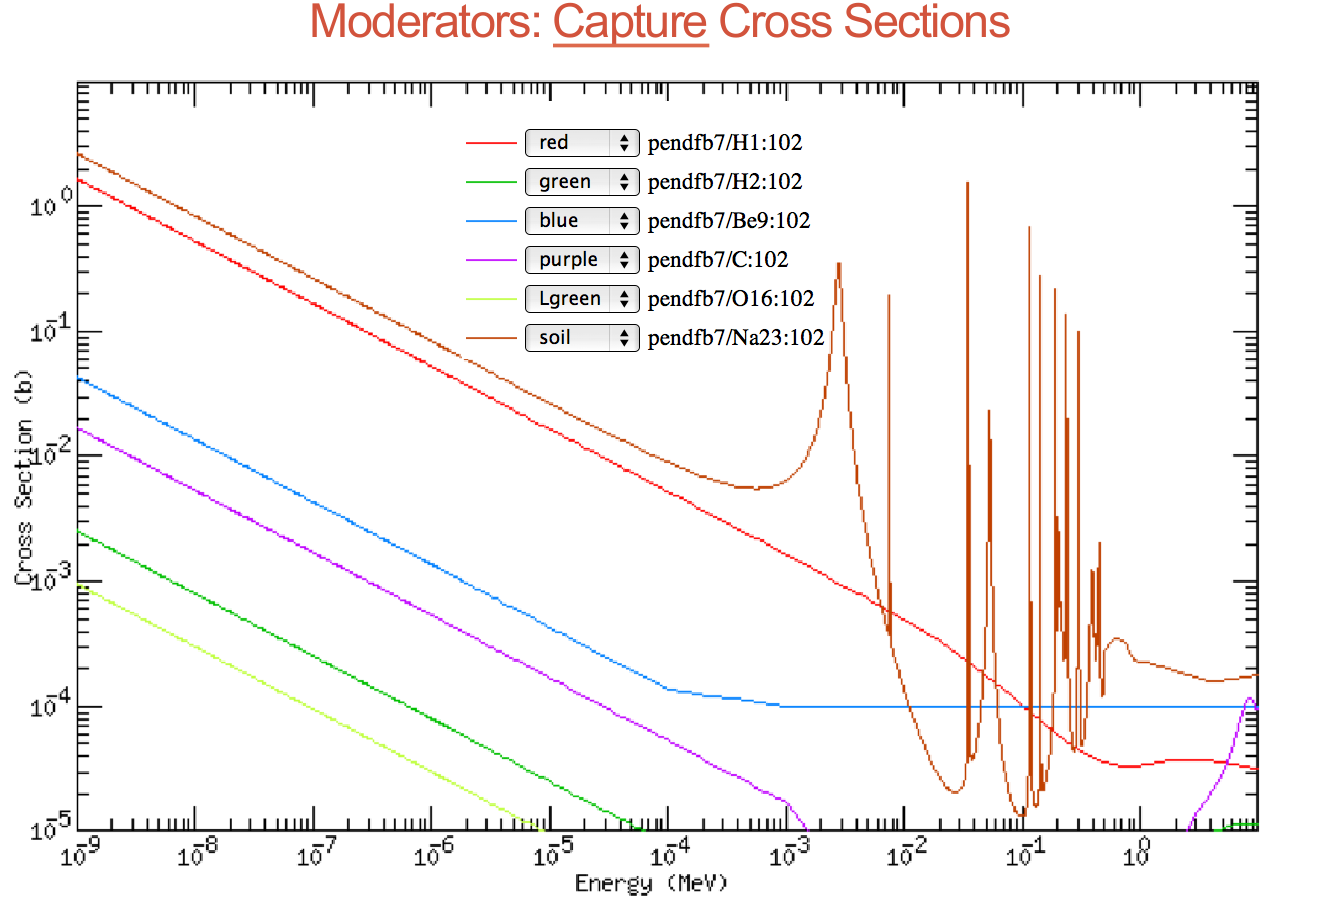
\includegraphics[width=4in]{images/capture-xs.png}
  \\
  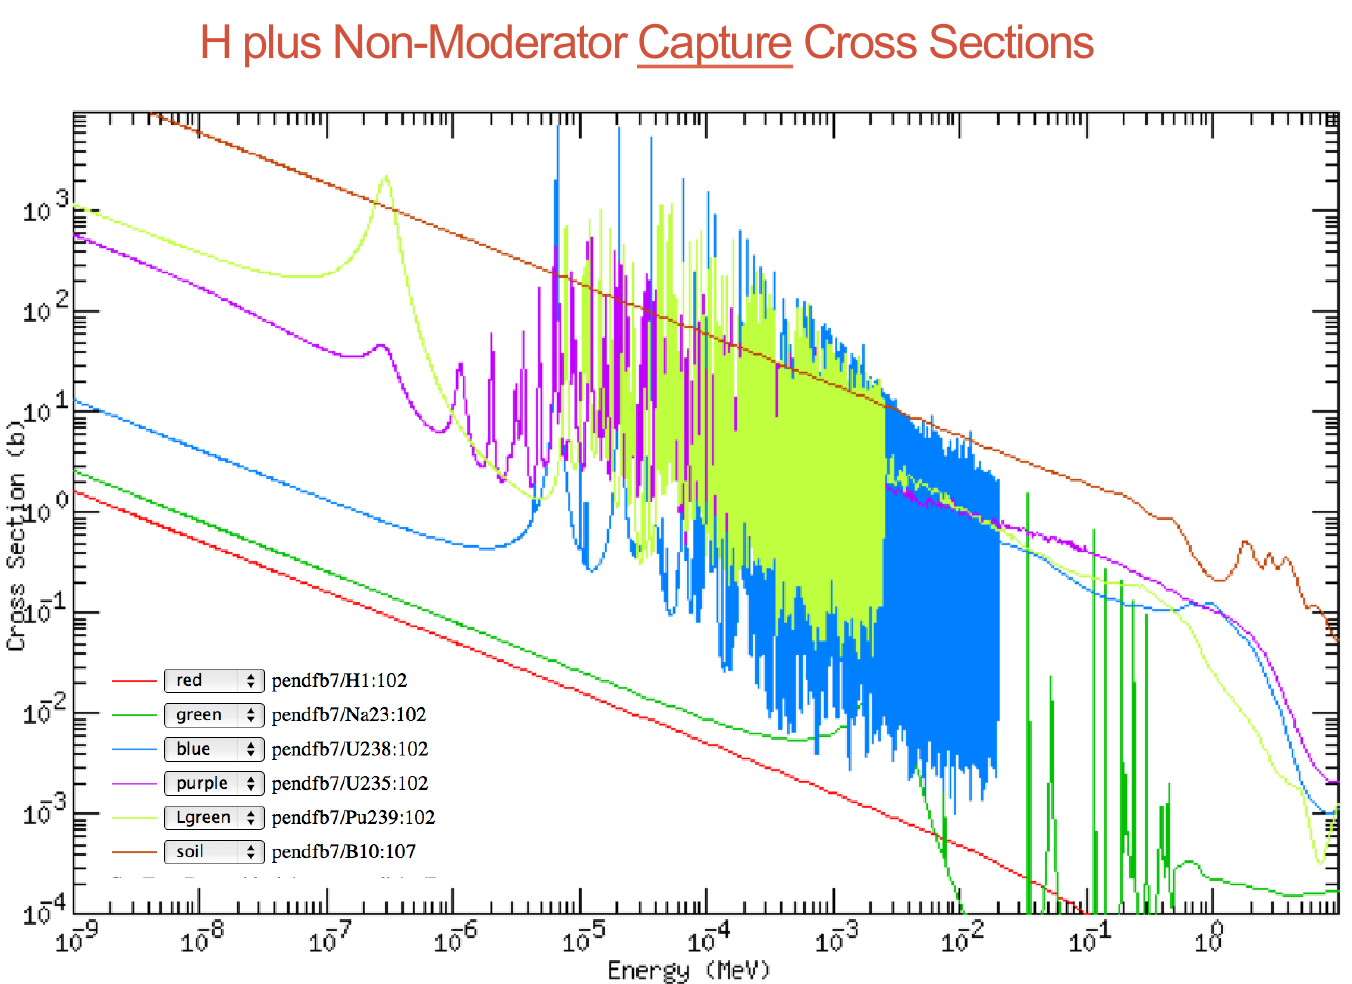
\includegraphics[width=4in]{images/capture-xs-2.png}
  \caption{Capture Cross Section} \label{capture-xs}
\end{figure}
\begin{enumerate}
\item H has no resonance; it has the highest scattering xs in LWR, so we can ignore any other isotopic's neutron scattering.   
\item Na has a huge resonance in 23 keV, and more resonances at higher energies because it is a heavy isotope.
\item Near zero energy,
\eqn{ \sigma(E\to 0) = }
\item Resonance at 6 to 7 eV: U238. 
\item U235's thermal elastic xs is larger than 238's, and they both have resonance around the same range.   
\item A small resonance at .3 eV: Pu239 (its signiture is a super low energy scattering xs). 
\end{enumerate}

\item Given an unknown material type, all we care is to count the nucleus density of each material and look at it's xs. 
\item Average fission neutron energy: 2 MeV; average peak fission energy: 1 MeV; see fission sepctrum. 

\item Core decay heat after 1 day is about 1\% rated. 


\end{enumerate}
%%%%%%%%%%%%%%%%%%%%%%%%% Qualify Exam End %%%%%%%%%%%%%%%%%%%%%%%%%%%%


\end{document}
